% !TEX root = ../CourseOT.tex

%%%%%%%%%%%%%%%%%%%%%%%%%%%%%%%%%%%%%%%%%%%%%%%%%%%%%%%%%%%%%%%%%%%%%%%%%%%
%%%%%%%%%%%%%%%%%%%%%%%%%%%%%%%%%%%%%%%%%%%%%%%%%%%%%%%%%%%%%%%%%%%%%%%%%%%
%%%%%%%%%%%%%%%%%%%%%%%%%%%%%%%%%%%%%%%%%%%%%%%%%%%%%%%%%%%%%%%%%%%%%%%%%%%
\section{Extensions}

%%%%%%%%%%%%%%%%%%%%%%%%%%%%%%%%%%%%%%%%%%%%%%%%%%%%%%%%%%%%%%%%%%%%%%%%%%%
\subsection{Dynamical formulation}

%%%%%%%%%%%%%%%%%%%%%%%%%%%%%%%%%%%%%%%%%%%%%%%%%%%%%%%%%%%%%%%%%%%%%%%%%%%
\subsection{Unbalanced OT}

%%%%%%%%%%%%%%%%%%%%%%%%%%%%%%%%%%%%%%%%%%%%%%%%%%%%%%%%%%%%%%%%%%%%%%%%%%%
\subsection{Gromov Wasserstein}


Optimal transport needs a ground cost $\C$ to compare histograms $(\a,\b)$, it can thus not be used if the histograms are not defined on the same underlying space, or if one cannot pre-register these spaces to define a ground cost. 
%
To address this issue, one can instead only assume a weaker assumption, namely that one has at its disposal two matrices $\distD \in \RR^{n \times n}$ and $\distD' \in \RR^{m \times m}$ that represent some relationship between the points on which the histograms are defined. A typical scenario is when these matrices are (power of) distance matrices.
%
The Gromov-Wasserstein problem reads
\eql{\label{eq-gw-def}
	\GWD( (\a,\distD), (\b,\distD') )^2 \eqdef
	\umin{ \P \in \CouplingsD(\a,\b) } 
		\Ee_{\distD,\distD'}(\P) \eqdef 
		\sum_{i,j,i',j'} |\distD_{i,i'} - \distD'_{j,j'}|^2 \P_{i,j}\P_{i',j'}.  
}
This is a non-convex problem, which can be recast as a Quadratic Assignment Problem (QAP)~\cite{loiola-2007} and is in full generality NP-hard to solve for arbitrary inputs. 
%
It is in fact equivalent to a graph matching problem~\cite{lyzinski-2015} for a particular cost.

One can show that $\GWD$ satisfies the triangular inequality, and in fact it defines a distance between metric spaces equipped with a probability distribution (here assumed to be discrete in definition~\eqref{eq-gw-def}) up to isometries preserving the measures.
%
This distance was introduced and studied in details by Memoli in~\cite{memoli-2011}. An in-depth mathematical exposition (in particular, its geodesic structure and gradient flows) is given in~\cite{SturmGW}. See also~\cite{schmitzer2013modelling} for applications in computer vision.
%
This distance is also tightly connected with the Gromov-Hausdorff distance~\cite{gromov-2001} between metric spaces, which have been used for shape matching~\cite{memoli-2007,bronstein-2010}. 



%%%%%%%%%%%%%%%%%%%%%
\begin{rem}{Gromov-Wasserstein distance}
	The general setting corresponds to computing couplings between metric measure spaces $(\X,\dist_\X,\al_\X)$
	and $(\Y,\dist_\Y,\al_\Y)$ where $(\dist_\X,\dist_\Y)$ are distances and $(\al_\X,\al_\Y)$ are measures on their respective spaces.
	%
	One defines 
	\begin{align}
		\label{eq-gw-generic}
		\GW( (\al_\X,\dist_\X), (\al_\Y,\dist_\Y) )^2 \eqdef 
		\umin{ \pi \in \CouplingsD(\al_\X,\al_Y) } 
		\int_{\X^2 \times \Y^2}
		| \dist_\X(x,x')-\dist_\Y(y,y') |^2
		\d\pi(x,y)\d\pi(x',y').
	\end{align}
	$\GW$ defines a distance between metric measure spaces up to isometries, where one says that $(\al_\X,\dist_\X)$ and $(\al_\Y,\dist_\Y) $ are isometric if there exists $\phi : \X \rightarrow \Y$ such that $\phi_{\sharp}\al_\X=\al_\Y$ and $\dist_\Y(\phi(x),\phi(x'))=\dist_\X(x,x')$.
\end{rem}
%%%%%%%%%%%%%%%%%%%%%



%%%%%%%%%%%%%%%%%%%%%
\begin{rem}{Gromov-Wasserstein geodesics}
The space of metric spaces (up to isometries) endowed with this $\GW$ distance~\eqref{eq-gw-generic} has a geodesic structure. \cite{SturmGW} shows that the geodesic between  $(\X_0,\dist_{\X_0},\al_0)$ and $(\X_1,\dist_{\X_1},\al_1)$ can be chosen to be 
$t \in [0,1] \mapsto (\X_0 \times \X_1,\dist_t,\pi^\star)$ where $\pi^\star$ is a solution of~\eqref{eq-gw-generic} and for all $((x_0,x_1), (x_0',x_1')) \in (\X_0 \times \X_1)^2$, 
\eq{
	\dist_t((x_0,x_1), (x_0',x_1')) \eqdef
	(1-t)\dist_{\X_0}(x_0,x_0') + t\dist_{\X_1}(x_1,x_1').
}
This formula allows one to define and analyze gradient flows which minimize functionals involving metric spaces, see~\cite{SturmGW}. It is however difficult to handle numerically, because it involves computations over the product space $\X_0 \times \X_1$. 
%
A heuristic approach is used in~\cite{peyre2016gromov} to define geodesics and barycenters of metric measure spaces while imposing the cardinality of the involved spaces and making use of the entropic smoothing~\eqref{eq-gw-entropy} detailed below.
\end{rem}
%%%%%%%%%%%%%%%%%%%%%

To approximate the computation of $\GWD$, and to help convergence of minimization schemes to better minima, one can consider the entropic regularized variant
\eql{\label{eq-gw-entropy}
	\umin{ \P \in \CouplingsD(\a,\b) } 
		\Ee_{\distD,\distD'}(\P) - \epsilon \HD(\P).
}
As proposed initially in~\cite{gold-1996,rangarajan-1999}, and later revisited in~\cite{2016-solomon-gw} for applications in graphics, one can use iteratively Sinkhorn's algorithm to progressively compute a stationary point of~\eqref{eq-gw-entropy}. 
%
Indeed, successive linearizations of the objective function lead to consider the succession of updates
\eql{\label{eq-gw-sinkh}
	\itt{\P} \eqdef \umin{ \P \in \CouplingsD(\a,\b) } \dotp{\P}{\it{\C}} - \epsilon\H(\P)
		\qwhereq
}
\eq{
		\it{\C} \eqdef \nabla \Ee_{\distD,\distD'}(\it{\P}) = -\transp{\distD'} \it{\P} \distD, 
}
which can be interpreted as a mirror-descent scheme~\cite{2016-solomon-gw}. Each update can thus be solved using Sinkhorn iterations~\eqref{eq-sinkhorn} with cost $\it{\C}$. Figure~\eqref{fig-gw} illustrates the use of this entropic Gromov-Wasserstein to compute soft maps between domains. 


\begin{figure}
\centering
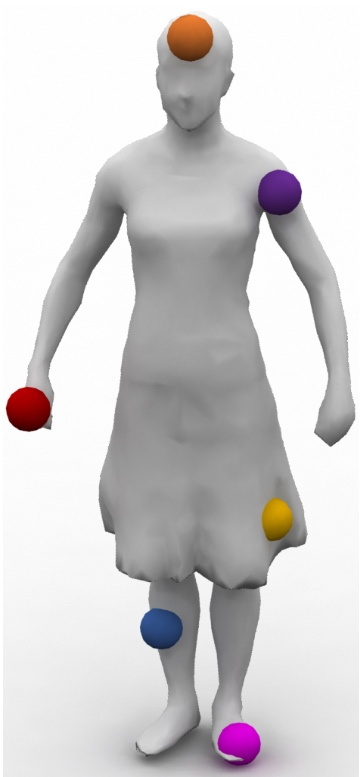
\includegraphics[height=.22\linewidth]{gw/source}
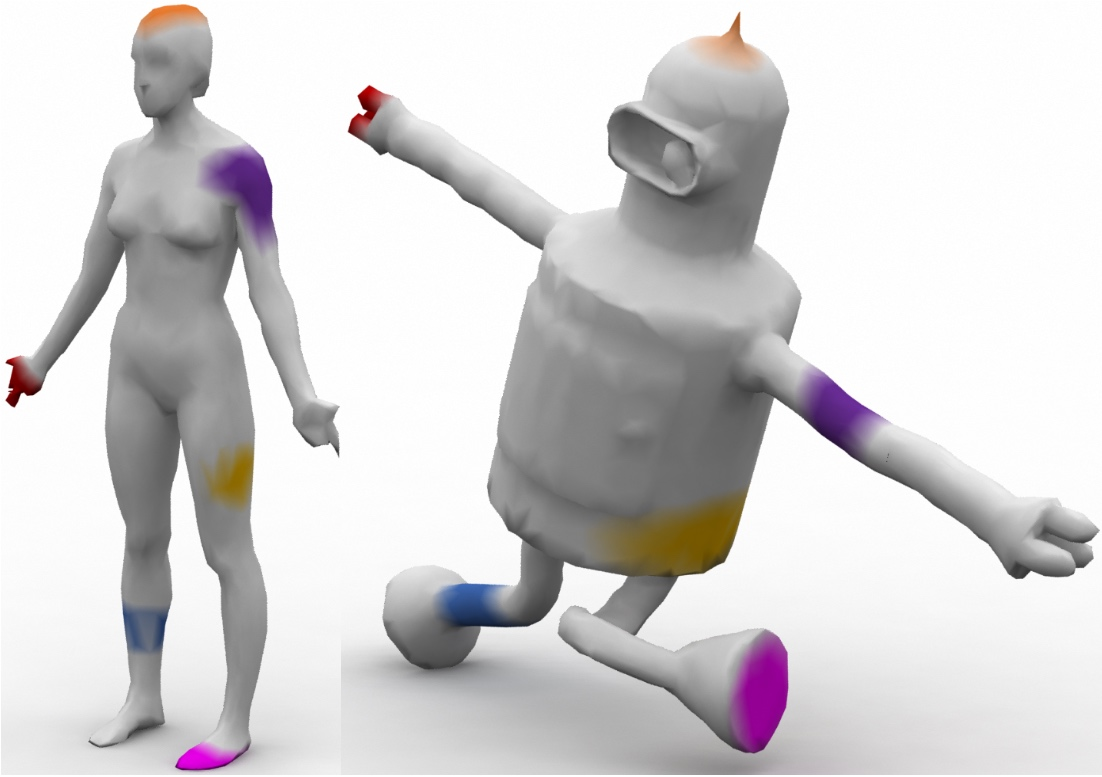
\includegraphics[height=.22\linewidth]{gw/target-surf}
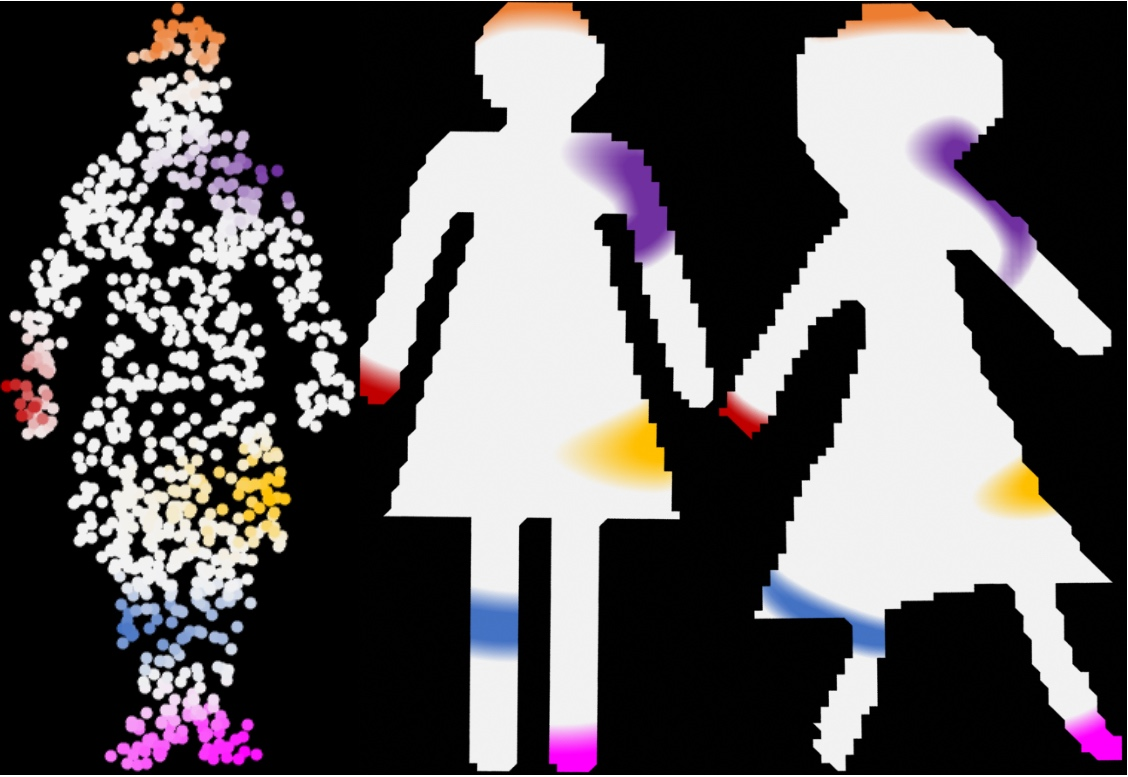
\includegraphics[height=.22\linewidth]{gw/target-2d}
\caption{\label{fig-gw}
Example of fuzzy correspondences computed by solving GW problem~\eqref{eq-gw-entropy} with Sinkhorn iterations~\eqref{eq-gw-sinkh}. Extracted from~\cite{2016-solomon-gw}.
}
\end{figure}


%%%%%%%%%%%%%%%%%%%%%%%%%%%%%%%%%%%%%%%%%%%%%%%%%%%%%%%%%%%%%%%%%%%%%%%%%%%
\subsection{Quantum OT}

Static formulation.

Gurvits algorithm, Q-sinkhorn.